\chapter{再入段运动特性分析与弹道设计}
\thispagestyle{empty}

\section{再入段运动方程}

\subsection{矢量形式段动力学方程}

空间质心运动方程段矢量形式为
\begin{equation}
	m \dfrac{\d^2 \bm{r}}{\d t^2} = \bm{P} + \bm{R} + \bm{F}_{c} +m\bm{g} + \bm{F}'_k
\end{equation}
由于再入段不考虑推力、控制力及附加哥氏力(无质量变化)等作用,则质心运动矢量方程为
\begin{equation}
	m \dfrac{\d^2 \bm{r}}{\d t^2} = \bm{R} + m\bm{g}
\end{equation}

在体坐标系中建立的绕质心动力学方程为
\begin{equation}
	\bm{I}\cdot \dfrac{\d \bm{\omega}_T}{\d t} + \bm{\omega}_T\times(\bm{I}\cdot \bm{\omega}_T) = \bm{M}_{st} + \bm{M}_c + \bm{M}_d + \bm{M}'_k+\bm{M}'_{rel}
\end{equation}
当不考虑控制力矩、附加哥氏力矩(无质量变化)等作用时,矢量方程为
\begin{align}
	\bm{I}\cdot \dfrac{\d \bm{\omega}_T}{\d t} + \bm{\omega}_T\times(\bm{I}\cdot \bm{\omega}_T) &= \bm{M}_{st} + \bm{M}_d \\
	\bm{\omega}_T = \bm{\omega} + \bm{\omega}_e
\end{align}
其中,$\bm{\omega}$为飞行器姿态相对于发色坐标系的转动角速度,$\bm{\omega_e}$为地球自转角速度。


\subsection{地面发射坐标系中再入段空间运动方程}
可将矢量运动方程分解到发射系中,也可直接利用空间运动方程进行简化得到:

\noa[1] 无动力,推力为0。
\begin{equation}
	P = 0
\end{equation}

\noa[2] 无控制,不考虑控制偏转角及控制力。
\begin{align}
	X_{\text{1\c}} = Y_{2\c} = Z_{3\c} = 0\\
	\delta_\varphi = \delta_\psi = \delta_\gamma = 0
\end{align}

\noa[3] 无质量消耗,为理想的常质量质点系。
\begin{align}
	\dot{m} &= 0 \\
	\dot{I}_{x1} = \dot{I}_{y1} &= \dot{I}_{z1} = 0
\end{align}

\noa[4] 飞行时间短,可忽略地球自转对相对角速率对影响。
\begin{equation}
	\begin{bmatrix}
		\omega_{Tx1} \\
		\omega_{Ty1}\\
		\omega_{Tz1}
	\end{bmatrix}
	=
	\begin{bmatrix}
		\omega_{x1} \\
		\omega_{y1} \\
		\omega_{z1}
	\end{bmatrix}
	\qquad 
	\begin{bmatrix}
		\varphi_T \\
		\psi_T \\
		\gamma_T
	\end{bmatrix}
	=
	\begin{bmatrix}
		\hspace*{0.1em}\varphi \hspace*{0.1em}\\
		\hspace*{0.1em}\psi \hspace*{0.1em}\\
		\hspace*{0.1em}\gamma \hspace*{0.1em}
	\end{bmatrix}
\end{equation}
则得到简化后的22个方程为
\begin{equation}
	\begin{cases}
		\, m 
		\begin{bmatrix}
			\dfrac{\d v_x}{\d t} \\[0.5em]
			\dfrac{\d v_y}{\d t} \\[0.5em]
			\dfrac{\d v_z}{\d t}
		\end{bmatrix}
		= G_V
		\begin{bmatrix}
			-X\\
			Y \\
			Z
		\end{bmatrix}
		+ m \dfrac{\dot{g}_r}{r}
		\begin{bmatrix}
			x  + R_{ox} \\
			y + R_{oy} \\
			z + R_{oz}
		\end{bmatrix}
		+ m \dfrac{g_{\omega e}}{\omega_e}
		\begin{bmatrix}
			\omega_{ex} \\
			\omega_{ey} \\
			\omega_{ez}
		\end{bmatrix}
		- m
		\begin{bmatrix}
			a_{11} & a_{12} & a_{13} \\
			a_{21} & a_{22} & a_{23} \\
			a_{31} & a_{32} & a_{33}
		\end{bmatrix}
		\begin{bmatrix}
			x  + R_{ox} \\
			y + R_{oy} \\
			z + R_{oz}
		\end{bmatrix}
		 - m
		 \begin{bmatrix}
		 	b_{11} & b_{12} & b_{13} \\
		 	b_{21} & b_{22} & b_{23} \\
		 	b_{31} & b_{32} & b_{33}
		 \end{bmatrix}
	 	\begin{bmatrix}
	 		v_x \\
	 		v_y \\
	 		v_z
	 	\end{bmatrix} 
 	\\[4em]
 	
 	\,  
 	\begin{bmatrix}
 		I_{x1} \dfrac{\d \omega_{x1}}{\d t} \\[0.5em]
 		I_{y1} \dfrac{\d \omega_{y1}}{\d t} \\[0.5em]
 		I_{z1} \dfrac{\d \omega_{z1}}{\d t}
 	\end{bmatrix}
 	+ 
 	\begin{bmatrix}
 		\big(I_{z1} - I_{y1}\big)\omega_{z1}\omega_{y1} \\
 		\big(I_{x1} - I_{z1}\big)\omega_{x1}\omega_{z1} \\
 		\big(I_{y1} - I_{x1}\big)
 	\end{bmatrix}
 	=
 	\begin{bmatrix}
 		0 \\
 		m_{y1\st}q S_M l_K \\
 		m_{z1\st}q S_M l_K 
 	\end{bmatrix}
 	+
 	\begin{bmatrix}
 		m_{x1}^{\overline{\omega}_{x1}}q S_M l_K\overline{\omega}_{x1}\\
 		m_{y1}^{\overline{\omega}_{y1}}q S_M l_K\overline{\omega}_{y1}\\
 		m_{z1}^{\overline{\omega}_{z1}}q S_M l_K\overline{\omega}_{z1}
 	\end{bmatrix}
 	\\[4em]
 	
 	\, 
 	\begin{bmatrix}
 		\dfrac{\d x}{\d t} \\[0.5em]
 		\dfrac{\d y}{\d t} \\[0.5em]
 		\dfrac{\d z}{\d t} 
 	\end{bmatrix}
	=
	\begin{bmatrix}
		v_x \\
		v_y \\
		v_z
	\end{bmatrix}
	\\[4em]
	
	\, 
	\begin{bmatrix}
		\omega_{x1} \\
		\omega_{y1} \\
		\omega_{z1}
	\end{bmatrix}
	=
	\begin{bmatrix}
		\dot{\gamma} - \dot{\varphi}\sin \psi \\
		\dot{\varphi}\cos \gamma + \dot{\varphi}\cos \psi \sin \gamma \\
		\dot{\varphi}\cos \psi \cos \gamma - \dot{\psi}\sin \gamma
	\end{bmatrix}
	\\[3.5em]
	
	\,
	\begin{cases}
		\, \theta = \arctan \big(v_y/ v_x\big) \\
		\, \sigma = - \arcsin(v_z /v)
	\end{cases}
	\\[2em]
	
	\,
	\begin{cases}
		\, \sin \beta = \cos\big(\varphi - \theta\big)\cos \sigma \sin \psi \cos \gamma + \sin \big(\varphi - \theta\big)\cos \sigma \sin \gamma - \sin \sigma \cos \psi \cos \gamma \\
		\, -\sin \alpha \cos \beta = \cos \big(\varphi - \theta\big)\cos \sigma \sin \psi \sin \gamma - \sin\big(\varphi - \theta\big) \cos \sigma \cos \gamma - \sin \sigma \cos \psi \sin \gamma \\
		\, \sin \nu = \dfrac{1}{\cos \sigma} \big(\cos \alpha \cos \psi \sin \gamma \big) - \sin \psi \sin \alpha 
	\end{cases}
	\\[3.2em]
	
	\, r = \sqrt{\big(x + R_{ox}\big)^2 + \big(y+R_{oy}\big)^2 + \big(z + R_{oz}\big)^2}
	\\[1em]
	
	\, \sin \phi = \dfrac{\big(x + R_{ox}\big)\omega_{ex} + \big(y + R_{oy}\big)\omega_{ey} + \big(z + R_{oz}\big)\omega_{ez}}{r\omega_e}
	\\[1em]
	
	\, R = \dfrac{a_e b_e}{\sqrt{a_e^2 \sin^2 \phi + b_e^2 \cos^2 \phi}}
	\\[1em]
	
	\, h = r - R
	\\
	
	v = \sqrt{v_x^2 + v_y^2 + v_z^2}
	\end{cases}
\end{equation}

\subsection{以总攻角、总升力表示的再入段空间弹道方程}

由于再入段飞行器可利用升力进行机动飞行,因此一些再入飞行器外形设计成升力体外形,不具有轴对称性,其法向气动力与横向气动力是不对称的。因此为充分利用升力体的机动能力,引入总升力与总攻角的概念。


\begin{figure}[!htb]
	\centering
	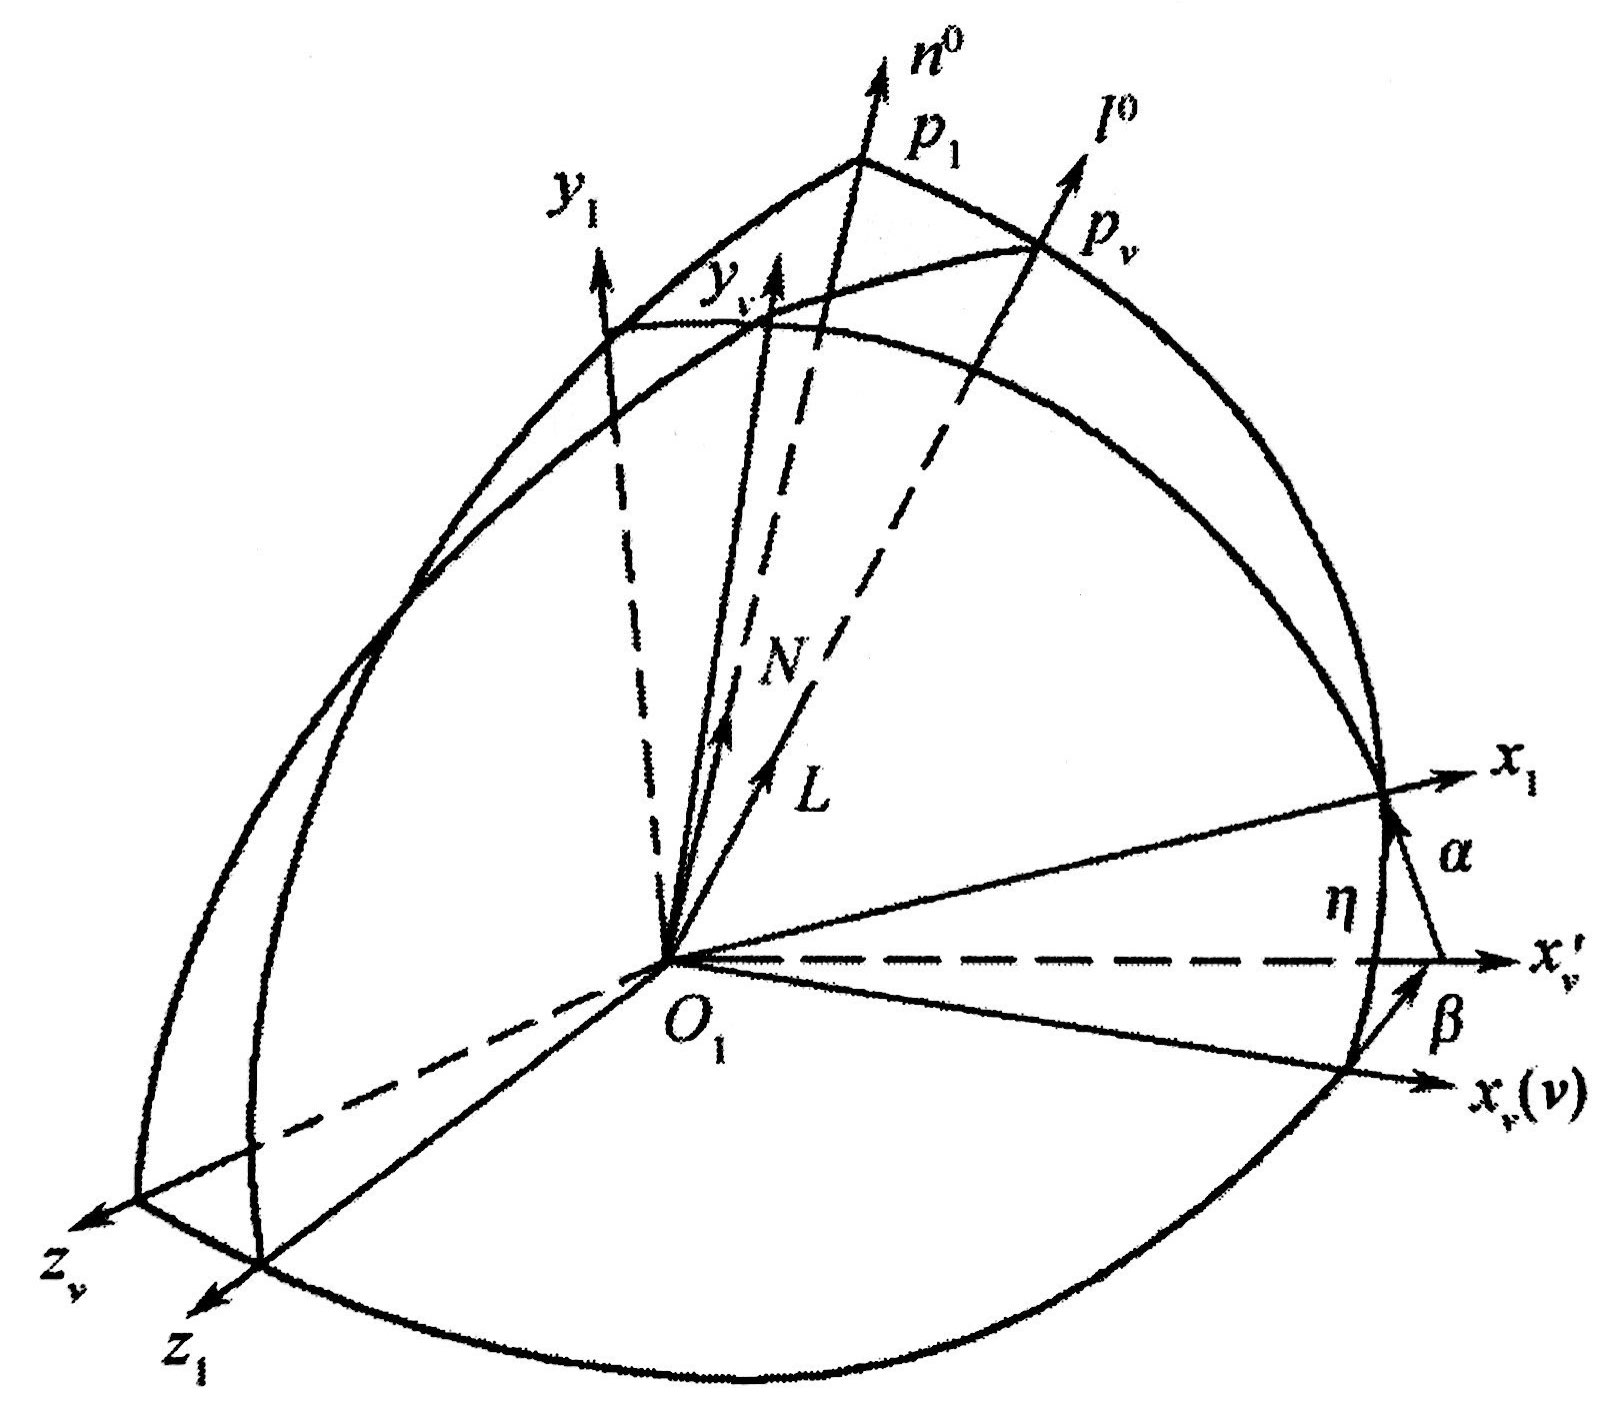
\includegraphics[width=0.4\linewidth]{pic/总攻角.jpg}
	\caption{总攻角$\eta$、总法向力$N$与总升力$L$}
	\label{总攻角}
\end{figure}

如图 \ref{总攻角} 所示,\dy[总攻角]{ZGJ}定义为速度轴$x_v$与弹体纵轴$x_1$的夹角,记作$\eta$,对应平面为总攻角平面。因此气动力可分解为
\begin{align}
	&\bm{R} = - X_1 \bm{x}_1^0 + N\bm{n}^0 \qquad \mbox{总法向力}N\mbox{垂直}\bm{x}_1\mbox{方向}\\
	&N\bm{n}^0 = Y_1\bm{y}_1^0 + Z_z \bm{z}_1^0 \qquad z_1o_1y_1\mbox{面与}x_1o_1x_v\mbox{面交线}O_1P_1
\end{align}

总攻角面内将气动力投影到速度系
\begin{align}
	&\bm{R} = - X\bm{x}_v^0 + L\bm{l}^0 \qquad \mbox{总法向力}N\mbox{垂直}\bm{x}_v\mbox{方向} \\
	&L\bm{l}^0 = Y \bm{y}_v^0 + Z \bm{z}_v^0 \qquad  z_vo_1y_v\mbox{面与}x_1o_1x_v\mbox{面交线}O_1P_v
\end{align}
下面给出引入总攻角后相关角度与力的相互关系:

\noa[1] 总攻角$\eta$与攻角$\alpha$、侧滑角$\beta$的关系
\begin{equation}
	\begin{cases}
		\, \cos \eta = \bm{x}_v^0 \cdot \bm{x}_1^0 \\
		\, \cos \alpha = \bm{x}_v^{'0}\cdot \bm{x}_z^0 \\
		\, \cos \beta = \bm{x}_v^0 \cdot \bm{x}_1^{'0}
	\end{cases}
\end{equation}
而速度轴与箭体轴之间存在转换关系,有
\begin{align*}
	\cos \eta &= \cos \alpha \cdot \cos \beta \\
	\sin^2 \eta &= \sin^2 \alpha + \sin^2 \beta - \sin^2 \alpha \sin^2 \beta 
\end{align*}
当攻角、侧滑角为小角度时,可以近似为
\begin{equation}
	\eta = \sqrt{\alpha^2 + \beta^2}
\end{equation}

\noa[2] 总法向力$N$与总升力$L$的关系

由于总法向力$N$和总升力$L$均在总攻角平面$x_1o_1x_v$内,则有
\begin{equation}
	\begin{cases}
		\, X = N \sin \eta + X_1 \cos \eta \\
		\, L = N \cos \eta - X_1 \sin \eta
	\end{cases}
\end{equation}

\begin{figure}[!htb]
	\centering
	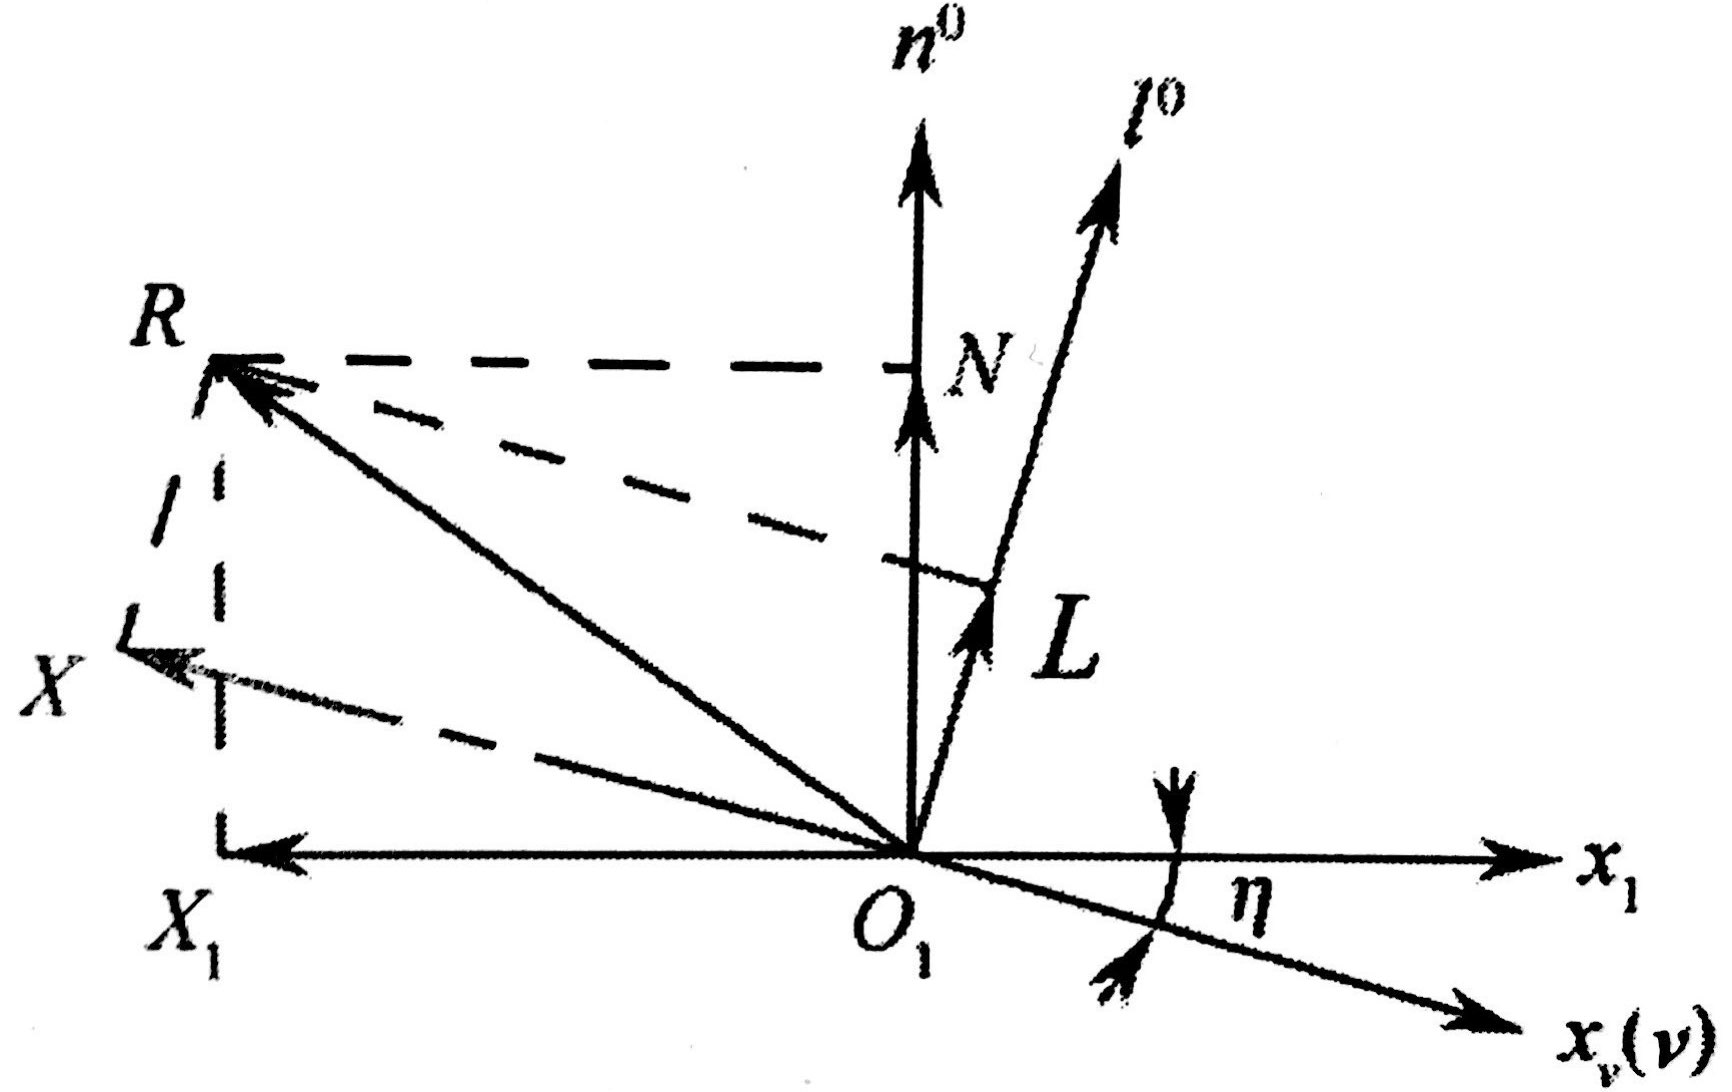
\includegraphics[width=0.4\linewidth]{pic/阻力.jpg}
	\caption{阻力$X$、总升力$L$与轴向力$X_1$、总法向力$N$的关系}
\end{figure}

若采用气动力系数描述,有
\begin{equation}
	\begin{cases}
		\, X = C_xqS_M \\
		\, X_1 = C_{x1} q S_M \\
		\, L = C_L q S_M \\
		\, N = C_N q S_M
	\end{cases}
	\quad \Longrightarrow \quad 
	\begin{cases}
		\, C_x = C_N \sin \eta + C_{x1} \cos \eta \\
		\, C_L = C_N \cos \eta - C_{x1} \sin \eta
	\end{cases}
\end{equation}
\red[注:有时候阻力系数可以用$C_D$表示,轴向力系数用$C_A$表示。]
\vspace*{0.5em}

\noa[3] 总法向力$N$与法向力$Y_1$、横向力$Z_1$关系
\begin{figure}[!htb]
	\centering
	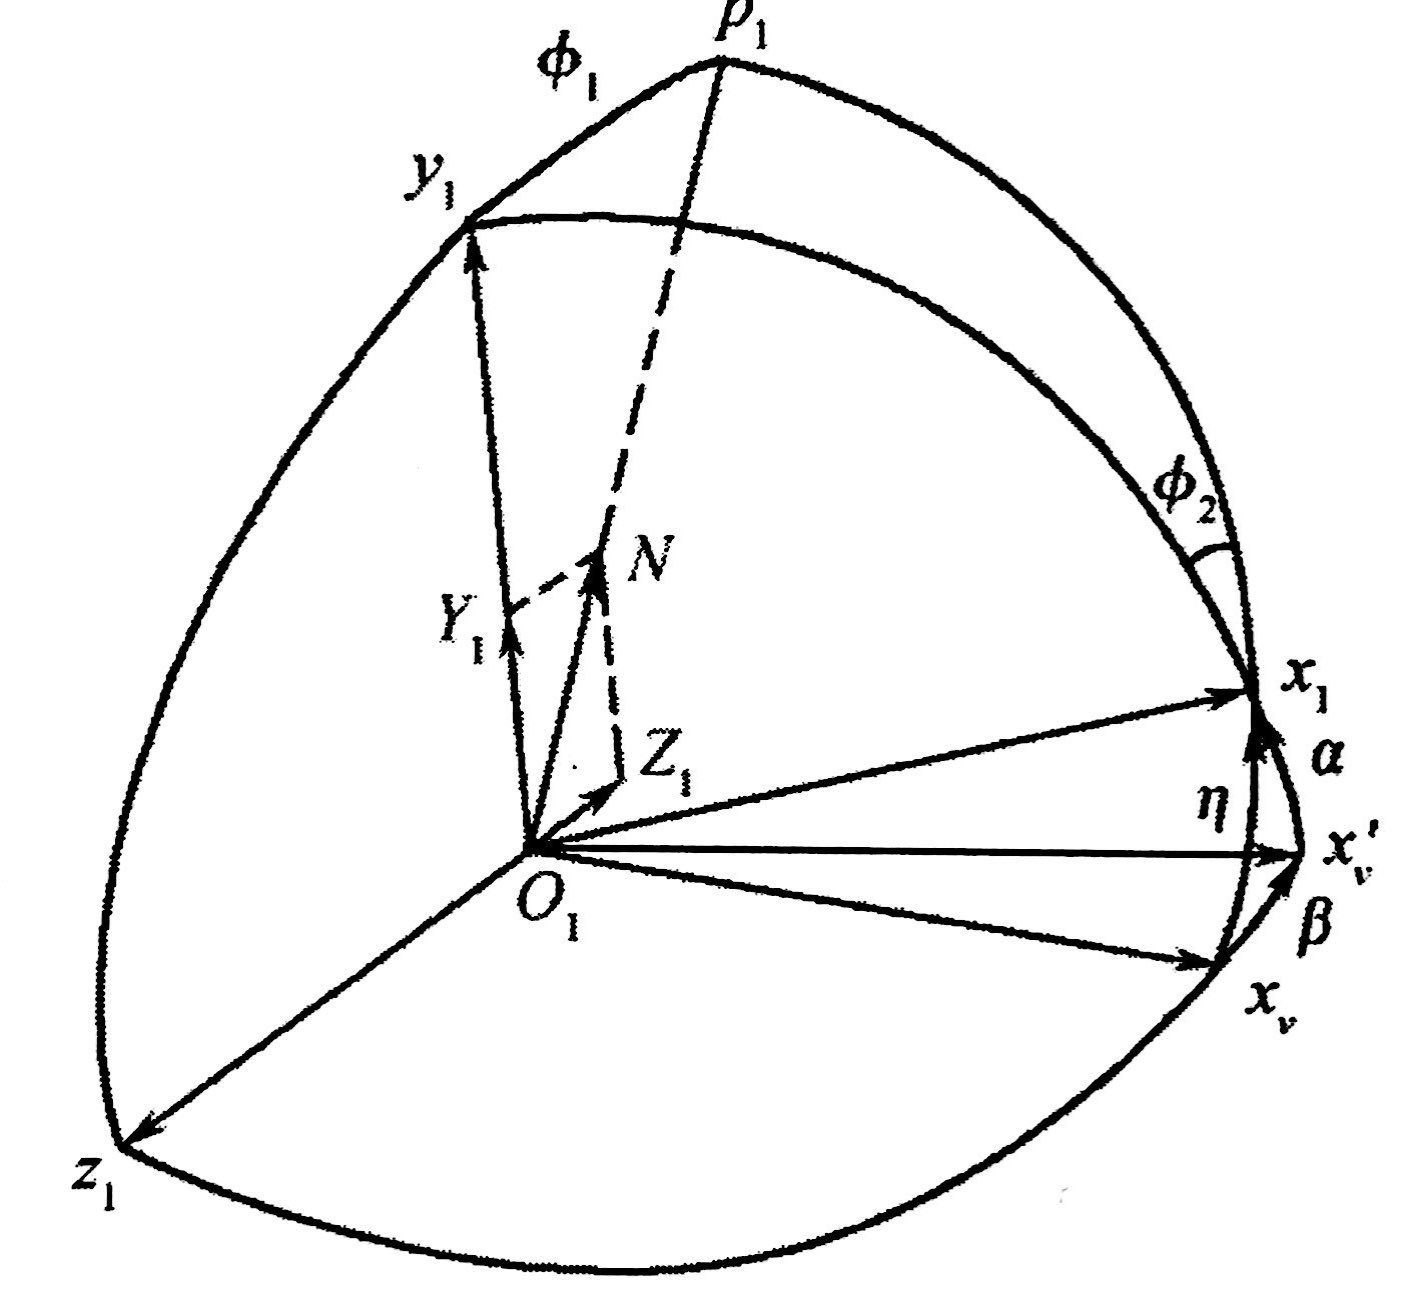
\includegraphics[width=0.4\linewidth]{pic/总法向力.jpg}
	\caption{总法向力$N$与法向力$Y_1$、横向力$Z_1$之间的关系}
\end{figure}
\vspace*{-1em}
\begin{equation}
	N \bm{n}^0 = Y_1\bm{y_1}^0 + Z_z \bm{z}_1^0 \qquad 
	\begin{cases}
		Y_1 = N \cos \phi_1 \\
		Z_1 = - N \sin \phi_1 
	\end{cases}
	\qquad 
	N^2 = Y_1^2 + Z_1^2
\end{equation}
\par 根据球面三角形公式,因为$o_1x_1$垂直于$y_1o_1p_1$平面,则
\begin{equation}
	\phi_1 = \phi_2
\end{equation}
由于在球面三角形$x_vx'_vx_1$中,$\angle x_vx'_v x_1 = 90 \degree$,所以球面三角形$x_vx'_vx_1$为球面直角三角形,则有
\par \blue[正弦公式]
\begin{equation}
	\sin \phi_2 = \dfrac{\sin \beta}{\sin \eta}
\end{equation}
\par \blue[余弦公式]
\begin{equation}
	\begin{cases}
		\, \cos \phi_2 = \dfrac{\cos \beta - \cos \alpha \cos \eta }{\sin \alpha \sin \eta}\\[0.5em]
		\, \cos \eta = \cos \beta \cdot \cos \alpha
	\end{cases}
	\quad \Rightarrow \quad 
	\cos \phi_2 = \dfrac{\sin \alpha \sin \beta}{\sin \eta}
\end{equation}

因此有法向力、横向力表达式
\begin{equation}
	\begin{cases}
		Y_1 = N \dfrac{\sin \alpha \sin \beta }{\sin \eta }\\[0.8em]
		Z_1 = -N \dfrac{\sin \beta}{\sin \eta}
	\end{cases}
	\qquad
	\begin{cases}
		C_{y1} = C_N \dfrac{\sin \alpha \sin \beta}{\sin \eta}\\[0.8em]
		C_{z1} = - C_N \dfrac{\sin \beta}{\sin \eta}
	\end{cases}
	\qquad
	C_N^2 = C_{y1}^2 + C_{z1}^2
\end{equation}
\vspace*{0.5em}

\noa[4] 总升力$L$与升力$Y$、侧力$Z$的关系
\begin{figure}[!htb]
	\centering
	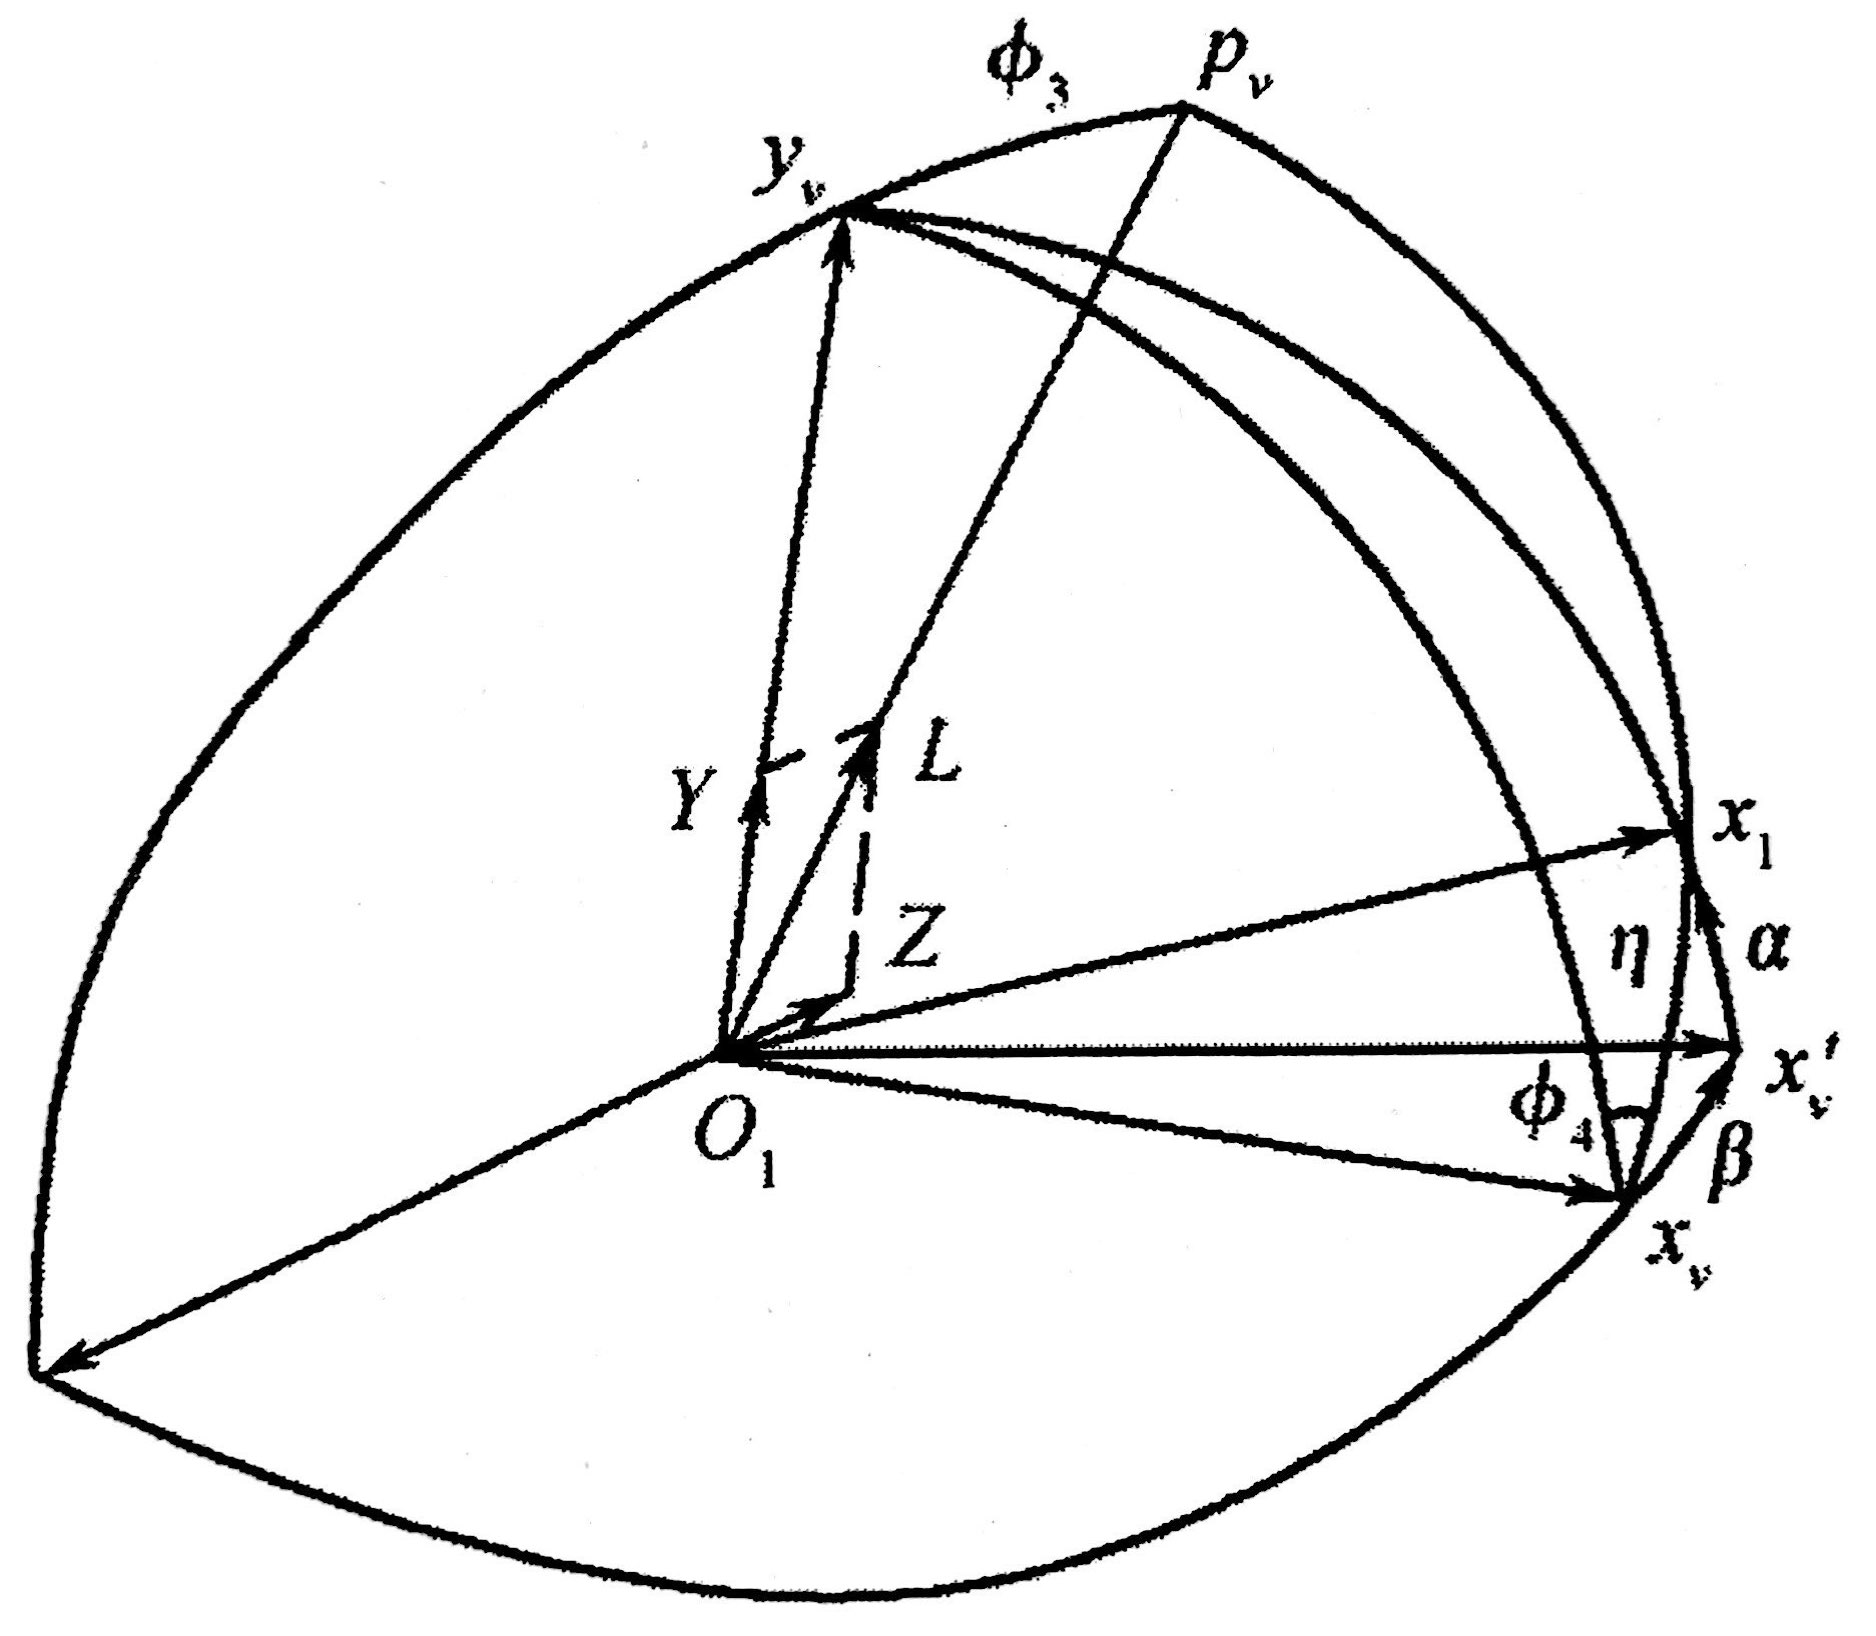
\includegraphics[width=0.4\linewidth]{pic/总升力.jpg}
	\caption{总升力$L$与升力$Y$、侧力$Z$的关系}
\end{figure}
\vspace*{-1em}
\begin{equation}
	L\bm{l}^0 = Y\bm{y}_v^0 + Z\bm{z}_v^0 \qquad 
	\begin{cases}
		\, Y = L \cos \phi_3 \\
		\, Z = - L \sin \phi_3
	\end{cases}
	\qquad 
	L^2 = Y^2 + Z^2
\end{equation}
根据球面三角形公式,有
\begin{equation}
	\phi_3 = \phi_4 = 90\degree - \angle x_1x_vx'_v
\end{equation}
而根据球面直角三角形,有
\begin{align}
	\cos \phi_4 &= \dfrac{\sin \alpha}{\sin \eta} \\[0.5em]
	\sin \phi_4 &= \dfrac{\cos \alpha \sin \beta}{\sin \eta}
\end{align}

因此有升力、侧力表达式为
\begin{equation}
	\begin{cases}
		\, Y = L \dfrac{\sin \alpha}{\sin \eta} \\[0.8em]
		\, Z = - L \dfrac{\cos \alpha \sin \beta}{\sin \eta}
	\end{cases}
	\qquad 
	\begin{cases}
		\, C_y = C_L \dfrac{\sin \alpha }{\sin \eta} \\[0.8em]
		\, C_z = - C_L \dfrac{\cos \alpha \sin \beta}{\sin \eta}
	\end{cases}
	\qquad 
	C_L^2 = C_y^2 + C_z^2
\end{equation}
\vspace*{0.5em}

\noa[4] 气动力$R$在发射系中的描述

\begin{equation}
	\bm{x}_1^0 = \cos \eta \bm{x}_v^0 + \sin \eta \bm{l}^0
\end{equation}
则
\begin{equation}
	\bm{R} = - X \bm{x}_v^0 + L \bm{l}^0 = - X\bm{x}_v^0 + \dfrac{L}{\sin \eta}\big(\bm{x}_1^0 - \cos \eta \bm{x}_v^0\big)
\end{equation}
\begin{figure}[!htb]
	\centering
	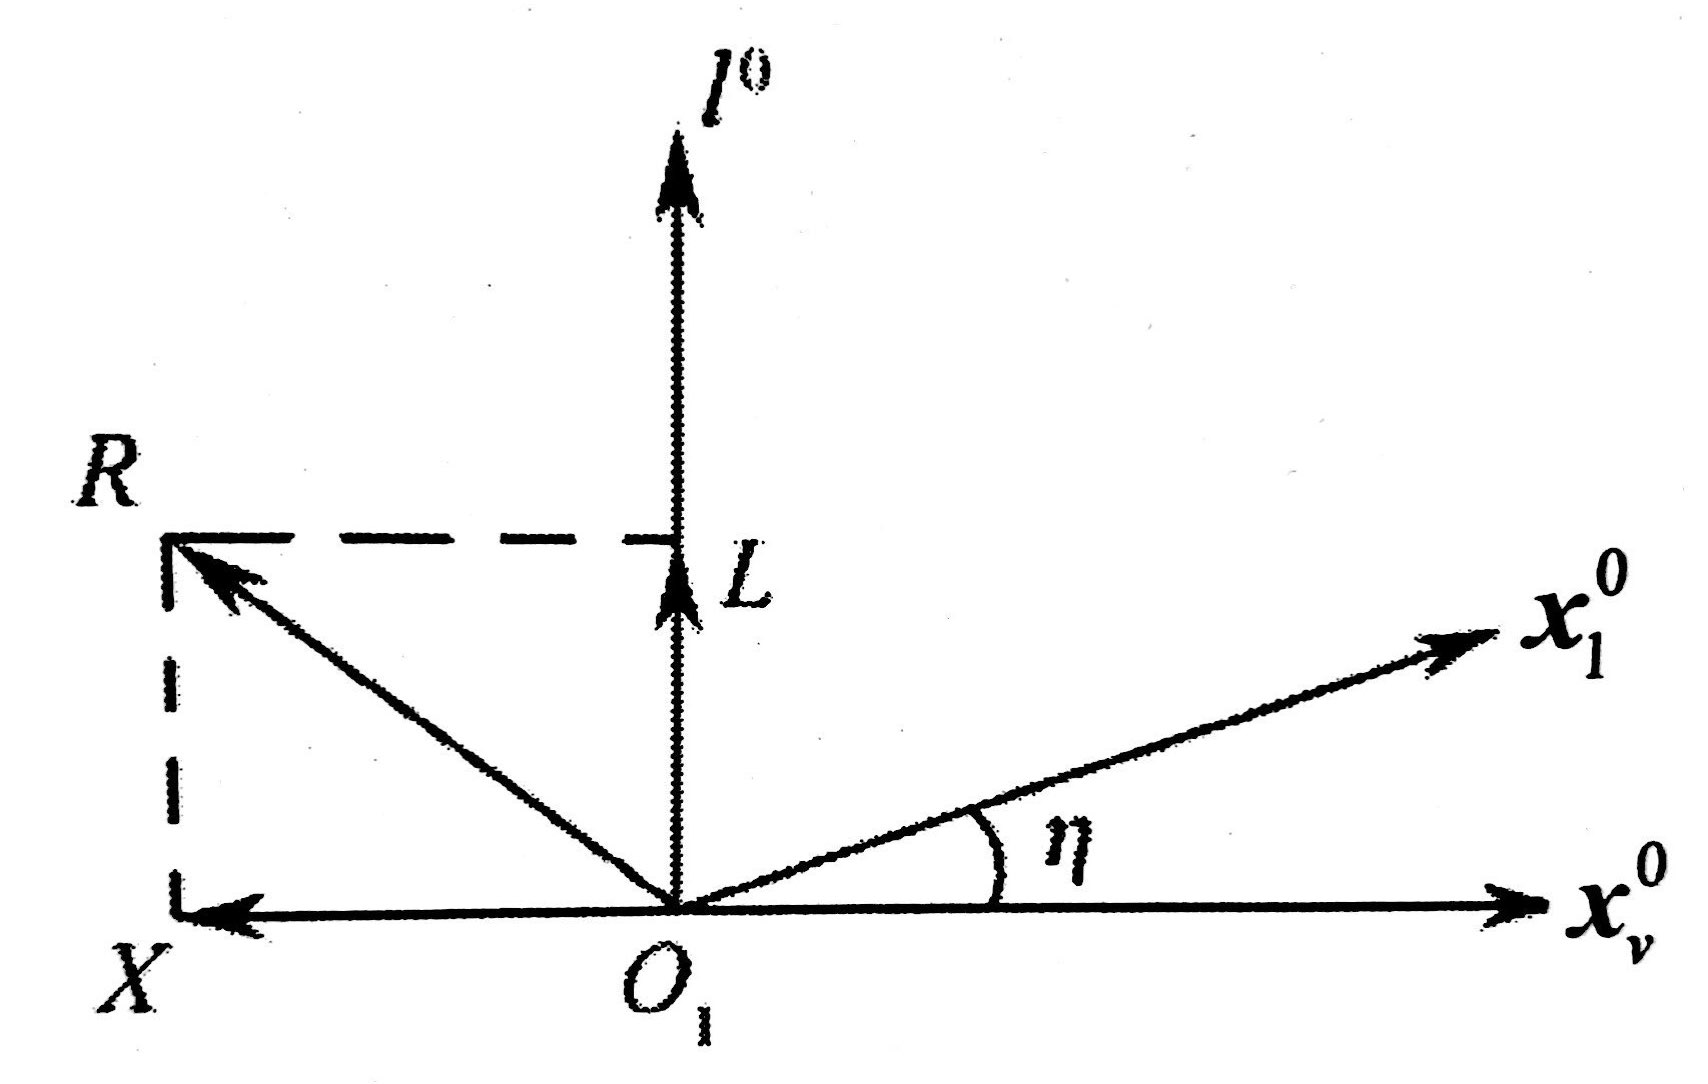
\includegraphics[width=0.4\linewidth]{pic/总气动力.jpg}
	\caption{单位矢量$\bm{l}^0$与$\bm{x}_1^0, \bm{x}_v^0$的关系}
\end{figure}

利用箭体系与发射系的方向余弦矩阵$\bm{G}_B$,有
\begin{equation}
	\bm{R} = 
	\begin{bmatrix}
		R_x \\
		R_y\\
		R_z
	\end{bmatrix}
	= -X
	\begin{bmatrix}
		\cos \theta \cos \sigma \\
		\sin \theta \cos \sigma \\
		- \sin \sigma
	\end{bmatrix}
	+ \dfrac{L}{\sin \eta}
	\begin{bmatrix}
		\cos \varphi \cos \psi - \cos \psi \cos \theta \cos \sigma \\
		\sin \varphi \cos \psi - \cos \eta \sin \theta \cos \sigma\\
		- \sin \psi + \cos \eta \sin \sigma
	\end{bmatrix}
\end{equation}
进一步可利用速度分解量简化计算,有
\begin{equation}
	\bm{v} = 
	\begin{bmatrix}
		v_x \\
		v_y \\
		v_z
	\end{bmatrix}
	= 
	-v
	\begin{bmatrix}
		\cos \theta \cos \sigma \\
		\sin \theta \cos \sigma \\
		- \sin \sigma 
	\end{bmatrix}
	\qquad 
	\bm{R} = -\dfrac{\red[X]}{v}
	\begin{bmatrix}
		v_x \\
		v_y\\
		v_z
	\end{bmatrix}
	+ \dfrac{\red[L]}{v \sin \red[\eta]}
	\begin{bmatrix}
		v \cos \varphi \cos \psi - \cos \red[\eta] v_x \\
		v \sin \varphi \cos \psi - \cos \red[\eta] v_y \\
		- v \sin \psi + \cos \red[\eta] v_z 
	\end{bmatrix}
\end{equation}
\vspace*{0.5em}

\noa[6] 稳定力矩描述

如果飞行器质心与压心均位于纵轴上,有
\begin{equation}
	\bm{M}_{st} = 
	\begin{bmatrix}
		M_{x1st}\\
		M_{y1st}\\
		M_{z1st}
	\end{bmatrix}
	=
	\begin{bmatrix}
		0 \\
		Z_1\big(x_p - x_g\big) \\
		-Y_1 \big(x_p - x_g\big)
	\end{bmatrix}
\end{equation}
代入
\begin{equation*}
	\begin{cases}
		\, Y_1 = N\dfrac{\sin \alpha \sin \beta}{\sin \eta}\\[0.8em]
		\, Z_1 = - N \dfrac{\sin \beta}{\sin \eta}
	\end{cases}
\end{equation*}
则
\begin{equation}
	\bm{M}_{st} = 
	\begin{bmatrix}
		M_{x1st}\\
		M_{y1st}\\
		M_{z1st}
	\end{bmatrix}
	=
	\begin{bmatrix}
		0 \\
		- m_n q S_M l_k \dfrac{\sin \beta}{\sin \eta} \\[0.8em]
		- m_n q S_M l_k \dfrac{\sin \alpha \cos \beta}{\sin \eta}
	\end{bmatrix}
\end{equation}
其中,$m_n = C_N \big(\overline{x}_p - \overline{x}_g\big)$为\dy[稳定力矩系数]{WDLJXS}。













